\documentclass[10pt,a4paper]{article}
\usepackage{amsmath}
\usepackage{amssymb}
\usepackage{graphicx}
\usepackage{color}
\usepackage{fancyhdr}
\usepackage{fancyvrb}
\usepackage[margin=3.5cm]{geometry}
\usepackage{framed}
\usepackage{enumerate}
\usepackage{textcomp}
\def\ket#1{\left|#1\right\rangle}
\def\bra#1{\left\langle#1\right|}
\def\braket#1{\left\langle#1\right\rangle}

\definecolor{linkcol}{rgb}{0.0, 0.0, 0.7}
\usepackage[colorlinks=true,urlcolor=linkcol,citecolor=black,linkcolor=linkcol]{hyperref}

\renewcommand{\theequation}{10.\arabic{equation}}
\setcounter{section}{10}
\renewcommand\thesection{\arabic{section}}
\renewcommand\thesubsection{\thesection.\arabic{subsection}}

\fancyhf{}
\lhead{\tiny Y.~D.~Chong (2021)}
\rhead{\scriptsize MH2801: Complex Methods for the Sciences}
\lfoot{}
\rfoot{\thepage}
\pagestyle{fancy}

\begin{document}
\setcounter{page}{77}

\noindent
{\Large \textbf{10. Fourier Series and Fourier Transforms}}
\vskip 0.2in

\label{fourier-series-and-fourier-transforms}

The \textbf{Fourier transform} is one of the most important
mathematical tools used for analyzing functions.  Given an arbitrary
function $f(x)$, with a real domain ($x \in \mathbb{R}$), we can
express it as a linear combination of complex waves.  The coefficients
of the linear combination form a counterpart to $f$, which is a
complex function $F(k)$ defined in a wave-number domain ($k \in
\mathbb{R}$). Often, $F$ turns out to be easier to deal with than
$f$. In particular, differential equations for $f$ can often be
reduced to algebraic equations for $F$, which are much easier to
solve.

\subsection{Fourier series}
\label{fourier-series}

We begin by discussing the \textbf{Fourier series}, which is used to
analyze functions that are periodic in their inputs.  A
\textbf{periodic function} $f(x)$ is a function of a real variable $x$
that repeats itself every time $x$ changes by $a$, as shown in the
figure below:

\begin{figure}[ht]
  \centering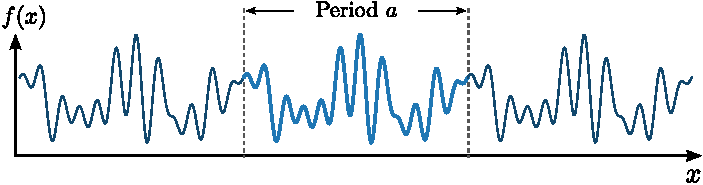
\includegraphics[width=0.7\textwidth]{periodicity}
\end{figure}

The constant $a$ is called the \textbf{period}.  We can write the
periodicity condition as
\begin{align}
  f(x+a) = f(x), \quad\forall\;\, x\in \mathbb{R}.
\end{align}
The value of $f(x)$ can be real or complex, but $x$ should be real.
You can think of $x$ as representing a spatial coordinate. We can also
think of the periodic function as being defined over a finite segment
$-a/2 \le x < a/2$, with periodic boundary conditions $f(-a/2) =
f(a/2)$. In spatial terms, this is like wrapping the segment into a
loop:

\begin{figure}[ht]
  \centering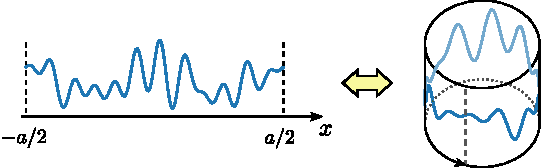
\includegraphics[width=0.65\textwidth]{periodic_ring}
\end{figure}

Let's consider what it means to specify a periodic function
$f(x)$. One way to specify the function is to give an explicit
mathematical formula for it. Another approach might be to specify the
function values in $-a/2 \le x < a/2$. Since there's an uncountably
infinite number of points in this domain, we can generally only
achieve an approximate specification of $f$ this way, by giving the
values of $f$ at a large but finite set $x$ points.

There is another interesting approach to specifying $f$. We can
express it as a linear combination of simpler periodic functions,
consisting of sines and cosines:
\begin{align}
  f(x) = \sum_{n=1}^\infty \alpha_n \sin\left(\frac{2\pi n x}{a}\right) + \sum_{m=0}^\infty \beta_m \cos\left(\frac{2 \pi m x}{a}\right).
\end{align}
(Note that the $n$ index does not include 0; since the sine term with
$n = 0$ vanishes for all $x$, it's redundant.) This is called a
\textbf{Fourier series}. Given the numbers $\{\alpha_n, \beta_m\}$,
which are called the \textbf{Fourier coefficients}, $f(x)$ can be
calculated for any $x$. The Fourier coefficients are real if $f(x)$ is
a real function, or complex if $f(x)$ is complex.

The justification for the Fourier series formula is that the sine and
cosine functions in the series are, themselves, periodic with period
$a$:
\begin{align}
  \sin\left(\frac{2\pi n (x+a)}{a}\right) = \sin\left(\frac{2\pi n x}{a} + 2\pi n\right) &= \sin\left(\frac{2\pi n x}{a}\right)\\
  \cos\left(\frac{2\pi m (x+a)}{a}\right) = \cos\left(\frac{2\pi m x}{a} + 2\pi m\right) &= \cos\left(\frac{2\pi m x}{a}\right).
\end{align}
Any linear combination of them thus automatically satisfies the
periodicity condition for $f$.

\subsubsection{Square-integrable functions}
\label{square-integrable-functions}

Can arbitrary periodic functions always be expressed as a Fourier
series? This question turns out to be surprisingly intricate, and its
resolution preoccupied mathematicians for much of the 19th
century. The full discussion is beyond the scope of this course.

Luckily, it turns out that a certain class of periodic functions,
commonly encountered in physical contexts, are guaranteed to always be
expressible as Fourier series. These are \textbf{square-integrable
  functions}, for which
\begin{align}
  \int_{-a/2}^{a/2} dx\; \big|\,f(x)\,\big|^2\;\;\text{exists and is finite}.
\end{align}
Unless otherwise stated, we will always assume that the functions
we're dealing with are square-integrable.

\subsubsection{Complex Fourier series and inverse relations}
\label{complex-fourier-series-and-inverse-relations}

We have written the Fourier series as sums over sine and cosine
functions. But as we know, sines and cosines can be re-written in
terms of exponentials by using Euler's formula. If we do this for the
Fourier series, it takes the form
\begin{align}
  f(x) = \sum_{n=-\infty}^\infty e^{2\pi i n x/a}\, f_n.
\end{align}
Now it is just a single sum, which is neater than having two separate
sums for sines and cosines. The sum includes negative integers $n$,
and involves a new set of complex Fourier coefficients, $\{f_n\}$. (As
an exercise, try working out how the old coefficients $\{\alpha_n,
\beta_n\}$ are related to the new coefficients $\{f_n\}$.)

If the Fourier coefficients $\{f_n\}$ are known, then $f(x)$ can be
calculated using the above formula.  The converse is also true: given
$f(x)$, we can determine the Fourier coefficients. To see how, observe
that
\begin{align}
  \int_{-a/2}^{a/2} dx \; e^{-2\pi i m x/a}\, e^{2\pi i n x/a} = a\, \delta_{mn}\quad \mathrm{for}\;m, n \in \mathbb{Z},
\end{align}
where $\delta_{mn}$ is the \textbf{Kronecker delta}, defined as:
\begin{align}
  \delta_{mn} = \left\{\begin{array}{ll}1, & \textrm{if}\; m = n\\ 0, & \mathrm{if}\;m\ne n.\end{array}\right.
\end{align}
Due to this property, the set of functions $\exp(2\pi i n x / a)$,
with integer values of $n$, are said to be \textbf{orthogonal}
functions.  (We won't go into the details now, but the term
``orthogonality'' is used here with the same meaning as in vector
algebra, where a set of vectors $\vec{v}_1, \vec{v}_2, \dots$ is said
to be orthogonal if $\vec{v}_m \cdot \vec{v}_n = 0$ for $m\ne n$.)
Hence,
\begin{align}
  \int_{-a/2}^{\,a/2} dx\; e^{-2\pi i m x/a} \;f(x)
  &= \, \int_{-a/2}^{\,a/2} dx\; e^{-2\pi i m x/a} \left[\sum_{n=-\infty}^\infty e^{2\pi i n x/a}\, f_n\right] \\
  &= \sum_{n=-\infty}^\infty \, \int_{-a/2}^{\,a/2} dx\; e^{-2\pi i m x/a}  \, e^{2\pi i n x/a} \;f_n \\
  &= \sum_{n=-\infty}^\infty \, a\, \delta_{mn} \, f_n \\
  &= a \,f_m.
\end{align}
The procedure of multiplying by $\exp(-2\pi i m x/a)$ and integrating
over $x$ acts like a sieve, filtering out all other Fourier components
of $f(x)$ and keeping only the one with the matching index $m$.  Thus,
we arrive at a pair of relations expressing $f(x)$ in terms of its
Fourier components, and vice versa:
\begin{align}
  f(x) &= \sum_{n=-\infty}^\infty e^{i k_n x}\, f_n, \quad \mathrm{where}\;\; k_n \equiv \frac{2\pi n}{a} \\
  f_n &= \displaystyle\,\frac{1}{a} \int_{-a/2}^{\,a/2} dx\; e^{-i k_n x}\, f(x).
  \label{eq:fn}
\end{align}
The real numbers $k_n$ are called \textbf{wave-numbers}.  They form a
discrete set, with one for each Fourier component.  In physics jargon,
we say that the wave-numbers are quantized to integer multiples of
$\Delta k \equiv 2\pi/a.$

\subsubsection{Example: Fourier series of a square wave}
\label{example-fourier-series-of-a-square-wave}

To get a feel for how the Fourier series behaves, let's look at a
square wave: a function that takes only two values $+1$ or $-1$,
jumping between the two values at periodic intervals.  Within one
period, the function is
\begin{align}
  f(x) = \left\{\begin{array}{ll}-1, & \;\;-a/2 \le x < 0 \\ +1, & \quad\;\;\; 0 \le x < a/2.\end{array}\right.
\end{align}
Plugging this into the Fourier relation, and doing the straightforward
integrals, gives the Fourier coefficients
\begin{align}
  f_n &= -i \, \frac{\left[\sin\left(n \pi/2\right)\right]^2}{n\pi/2 } \\
  &= \left\{\begin{array}{cl} -2i/n\pi ,& n \; \mathrm{odd} \\
  0,& n \; \mathrm{even}. \end{array}\right.
\end{align}
As can be seen, the Fourier coefficients become small for large $n$.
We can write the Fourier series as
\begin{align}
  f(x) \; \leftrightarrow \; \sum_{n=1,3,5,\dots} \frac{4\sin(2\pi n x / a)}{n \pi}.
\end{align}
If this infinite series is truncated to a finite number of terms, we
get an approximation to $f(x)$.

The plot below shows the graph of the square wave $f(x)$ alongside the
truncated Fourier series. As more terms are included in the truncated
Fourier series, the approximation gets better and better.

\begin{center}
  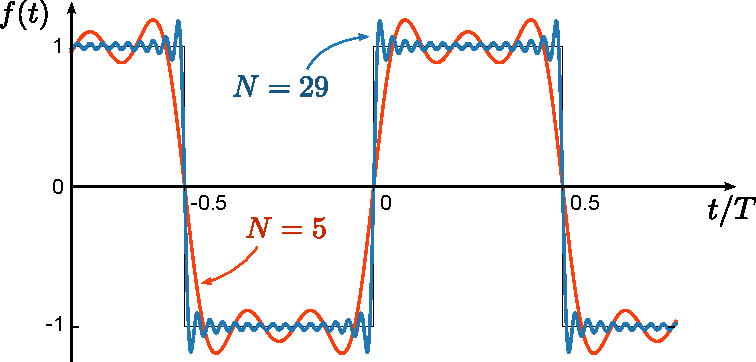
\includegraphics[width=0.6\textwidth]{square_fourier}
\end{center}

One amusing consequence of the above result is that we can use it to
derive a series expansion for $\pi$.  If we set $x = a/4$,
\begin{align}
  f(a/4) = 1 = \frac{4}{\pi} \left[\sin(\pi/2) + \frac{1}{3}\sin(3\pi/2) + \frac{1}{5}\sin(5\pi/2) + \cdots\right],
\end{align}
and hence
\begin{align}
  \pi = 4 \left(1 - \frac{1}{3} + \frac{1}{5} - \frac{1}{7} + \cdots\right).
\end{align}

\subsection{Fourier transforms}\label{fourier-transforms}

The Fourier series applies to periodic functions defined over the
interval $-a/2 \le x < a/2$.  But the concept can be generalized to
functions defined over the entire real line, $x \in \mathbb{R}$, if we
take the limit $a \rightarrow \infty$ carefully.

Suppose we have a function $f$ defined over the entire real line, $x
\in \mathbb{R}$, such that $f(x) \rightarrow 0$ for $x \rightarrow
\pm\infty$.  Imagine there is a family of periodic functions
$\big\{f_a(x) \,\big|\, a \in\mathbb{R}^+\big\}$, such that $f_a(x)$
has periodicity $a$, and approaches $f(x)$ in the limit $a\rightarrow
\infty$.  This is illustrated in the figure below:

\begin{figure}[ht]
  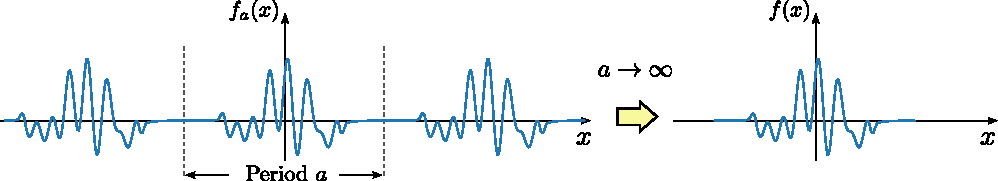
\includegraphics[width=0.99\textwidth]{periodicity_ft}
\end{figure}

In mathematical terms,
\begin{align}
  f(x) = \lim_{a \rightarrow \infty} f_a(x), \;\;\;\text{where}\;\; f_a(x+a) = f_a(x).
\end{align}
Since $f_a$ is periodic, it can be expanded as a Fourier series:
\begin{align}
  f_a(x) = \sum_{n=-\infty}^\infty e^{i k_n x}\, f_{an}, \quad\mathrm{where}\;\; k_n = n\Delta k, \;\; \Delta k = \frac{2\pi}{a}.
\end{align}
Here, $f_{an}$ denotes the $n$-th complex Fourier coefficient of the
function $f_a(x)$.  Note that each Fourier coefficient depends
implicitly on the periodicity $a$.

As $a \rightarrow \infty$, the wave-number quantum $\Delta k$ goes to
zero, and the set of discrete $k_n$ turns into a continuum.  During
this process, each Fourier coefficient $f_{an}$ goes to zero, because
there are more and more Fourier components in the vicinity of each $k$
value, and each individual component contributes less.  This implies
that we can replace the discrete sum with an integral. To accomplish
this, we multiply the summand by a factor of $(\Delta k/2\pi) /
(\Delta k/2\pi) = 1$:
\begin{align}
  f(x) = \lim_{a\rightarrow \infty} \left[\;\,\sum_{n=-\infty}^\infty \frac{\Delta k}{2\pi} \, e^{i k_n x}\, \left(\frac{2\pi \,f_{an}}{\Delta k} \right)\;\,\right].
\end{align}
(In case you're wondering, the choice of $2\pi$ factors is essentially
arbitrary; we are following the usual convention.) Next, define
\begin{align}
  F(k) \equiv \lim_{a \rightarrow \infty} \left[\frac{2\pi\, f_{an}}{\Delta k}\right]_{k = k_n}.
\end{align}
In the $a \rightarrow \infty$ limit, the $f_{an}$ in the numerator and
the $\Delta k$ in the denominator both go zero, but if their ratio
remains finite, the Fourier sum turns into an integral:
\begin{align}
  f(x) = \int_{-\infty}^{\infty} \frac{dk}{2\pi} \, e^{i k x}\, F(k).
\end{align}

\subsubsection{The Fourier relations}
\label{the-fourier-relations}

The function $F(k)$ is called the \textbf{Fourier transform} of
$f(x)$.  Just as we have expressed $f(x)$ in terms of $F(k)$, we can
also express $F(k)$ in terms of $f(x)$.  To do this, we apply the $a
\rightarrow \infty$ limit to Eq.~\eqref{eq:fn}:
\begin{align}
  F(k_n) &= \lim_{a\rightarrow \infty} \frac{2 \pi\, f_{an}}{\Delta k} \\
  &= \lim_{a\rightarrow \infty} \frac{2 \pi}{2\pi/a}\, \left(\frac{1}{a} \int_{-a/2}^{a/2} dx\; e^{-i k_n x}\right) \\
  &= \int_{-\infty}^\infty dx\; e^{-i kx}\, f(x).
\end{align}
Hence, we arrive at a pair of equations called the \textbf{Fourier
  relations}:
\begin{align}
  F(k) &= \;\int_{-\infty}^\infty dx\; e^{-ikx}\, f(x) \label{eq:ft}\\
  f(x) &= \int_{-\infty}^\infty \frac{dk}{2\pi}\; e^{ikx}\, F(k) \label{eq:ift}
\end{align}
Eq.~\eqref{eq:ft} is the Fourier transform, and Eq.~\eqref{eq:ift} is
called the \textbf{inverse Fourier transform}.

There are some differences between the two formulas.  First, $dk$ is
accompanied by a factor of $1/2\pi$, but there is no such factor for
$dx$; this is a matter of convention, tied to our earlier definition
of $F(k)$.  Second, the integral over $x$ contains a factor of
$e^{-ikx}$ but the integral over $k$ contains a factor of
$e^{ikx}$. One way to remember which equation has the positive sign in
the exponent is to interpret the inverse Fourier transform equation
(which has the form of an integral over $k$) as the continuum limit of
a sum over complex waves. In this sum, $F(k)$ plays the role of the
series coefficients, and the complex waves have the form $\exp(ikx)$
in accordance with our usual convention (see Chapter 6).

As noted in Section~\ref{square-integrable-functions}, all the
functions we deal with are assumed to be square integrable. This
includes the $f_a$ functions used to define the Fourier transform. In
the $a \rightarrow \infty$ limit, this implies that we are dealing
with functions such that
\begin{align*}
  \int_{-\infty}^{\infty} dx\; \big|\,f(x)\,\big|^2
\end{align*}
exists and is finite.

\subsubsection{A simple example}
\label{simple-example}

Consider the function
\begin{align}
  f(x) = \left\{\begin{array}{cl}e^{-\eta x}, & x \ge 0 \\ 0, & x < 0,\end{array}\right. \qquad \eta \in \mathbb{R}^+.
\end{align}
For $x < 0$, this is an exponentially-decaying function, and for $x <
0$ it is identically zero. The real parameter $\eta$ is called the
decay constant; for $\eta > 0$, the function $f(x)$ vanishes as $x
\rightarrow +\infty$ and can thus be shown to be
square-integrable. Larger values of $\eta$ correspond to faster
exponential decay.

The Fourier transform can be found by directly calculating the Fourier
integral:
\begin{align}
  F(k) \;=\; \;\int_{0}^\infty dx\; e^{-i kx}\, e^{-\kappa x} \;=\; \frac{-i}{k - i \eta}.
\end{align}
It is useful to plot the squared magnitude of the Fourier transform,
$|F(k)|^2$, against $k$.  This is called the \textbf{Fourier spectrum}
of $f(x)$.  In this case,
\begin{align}
  \big|\,F(k)\,\big|^2 = \frac{1}{k^2 + \eta^2}.
\end{align}
The Fourier spectrum is plotted below.  It consists of a peak centered
at $k = 0$, forming a curve called a \textbf{Lorentzian}.  The width
of the Lorentzian is dependent on the original function's decay
constant $\eta$. For small $\eta$, i.e. weakly-decaying $f(x)$, the
peak is narrow; for large $\eta$, i.e. rapidly-decaying $f(x)$, the
peak is broad.

\begin{figure}[h]
  \centering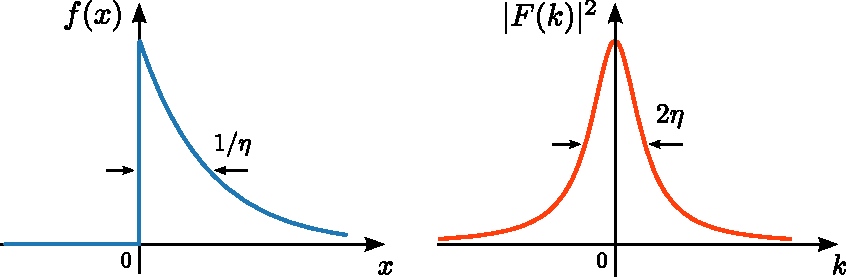
\includegraphics[width=0.69\textwidth]{fourier_example1}
\end{figure}

We can quantify the width of the Lorentzian by defining the
\textbf{full-width at half-maximum} (FWHM)---the width of the curve at
half the value of its maximum.  In this case, the maximum of the
Lorentzian curve occurs at $k=0$ and has the value of $1/\eta^2$.  The
half-maximum, $1/2\eta^2$, occurs when $\delta k = \pm \eta$.  Hence,
the original function's decay constant, $\eta$, is directly
proportional to the FWHM of the Fourier spectrum, which is $2\eta$.

To wrap up this example, let's evaluate the inverse Fourier transform:
\begin{align}
  f(x) \; = \; -i\int_{-\infty}^\infty \frac{dk}{2\pi} \; \frac{e^{i kx}}{k-i\eta}.
\end{align}
This can be solved by contour integration.  The analytic continuation
of the integrand has a simple pole at $k = i\eta$.  For $x < 0$, the
numerator $\exp(ikx)$ vanishes far from the origin in the lower
half-plane, so we close the contour below.  This encloses no pole, so
the integral is zero.  For $x > 0$, the numerator vanishes far from
the origin in the upper half-plane, so we close the contour above,
with a counter-clockwise arc, and the residue theorem gives
\begin{align}
  f(x) = \left(\frac{-i}{2\pi}\right) \, \left(2\pi i\right) \, \mathrm{Res}\left[\, \frac{e^{ikx}}{k-i\eta}, \, k=i\eta\, \right] = e^{-\eta x} \qquad(\mathrm{for}\; x > 0),
\end{align}
in agreement with the form of $f(x)$ we started out with.

\subsection{Fourier transforms for time-domain functions}
\label{fourier-time}

So far, we have been dealing with functions of a spatial coordinate
$x$.  Of course, mathematical relations don't care about what kind of
physical variable we are dealing with, so the same equations could be
applied to functions of time $t$. However, there is a important
difference in \textit{convention}.  When dealing with functions of the
time coordinate $t$, it is customary to use a different sign
convention in the Fourier relations!

The Fourier relations for a function of time, $f(t)$, are:
\begin{align}
  \left\{\;\,\begin{aligned}F(\omega) &= \;\int_{-\infty}^\infty dt\; e^{i\omega t}\, f(t) \\ f(t) &= \int_{-\infty}^\infty \frac{d\omega}{2\pi}\; e^{-i\omega t}\, F(\omega).\end{aligned}\;\,\right.
\end{align}
Compared to the previously-derived Fourier relations,
Eqs.~\eqref{eq:ft} and \eqref{eq:ift}, the signs of the $\pm i \omega
t$ exponents are flipped.

There's a good reason for this difference in sign convention: it
arises from the need to describe propagating waves, which vary with
both space \textit{and} time.  As discussed in Chapter 6, a
propagating plane wave can be described by a wavefunction of the form
\begin{align}
  f(x,t) = A e^{i(kx - \omega t)},
\end{align}
where $k$ is the wave-number and $\omega$ is the angular frequency.
We write the plane wave function this way so that positive $k$
indicates forward propagation in space (i.e., in the $+x$ direction),
and positive $\omega$ indicates forward propagation in time (i.e., in
the $+t$ direction).  This requires the $kx$ and $\omega t$ terms in
the exponent to have opposite signs. Thus, when $t$ increases by some
amount, a corresponding \textit{increase} in $x$ leaves the exponent
unchanged.

As we have seen, the inverse Fourier transform relation describes how
a wave-form is broken up into a superposition of elementary waves.
For a wavefunction $f(x,t)$, the superposition is given in terms of
plane waves:
\begin{align}
  f(x,t) = \int_{-\infty}^\infty \frac{dk}{2\pi} \int_{-\infty}^\infty \frac{d\omega}{2\pi}\;\; e^{i(kx-\omega t)}\, F(k,\omega).
\end{align}
To be consistent with this, we need to treat space and time variables
with oppositely-signed exponents:
\begin{align}
  f(x) &= \int_{-\infty}^\infty \frac{dk}{2\pi}\; e^{ikx}\, F(k) \\
  f(t) &= \int_{-\infty}^\infty \frac{d\omega}{2\pi}\; e^{-i\omega t}\, F(\omega).
\end{align}
The other equations follow similarly.

\subsection{Basic properties of the Fourier transform}
\label{fourier-basic-properties}

The Fourier transform has several important properties.  These can all
be derived from the definition of the Fourier transform; the proofs
are left as exercises.

\begin{enumerate}
\item The Fourier transform is linear: if we have two functions $f(x)$
  and $g(x)$, whose Fourier transforms are $F(k)$ and $G(k)$
  respectively, then for any constants $a, b \in \mathbb{C}$,
  \begin{align}
    a f(x) + b g(x) \;\;\; \overset{\mathrm{FT}}{\longrightarrow} \;\;\;
    a F(k) + b G(k).
  \end{align}
  
\item Performing a coordinate translation on a function causes its
  Fourier transform to be multiplied by a phase factor:
  \begin{align}
    f(x+b) \;\;\; \overset{\mathrm{FT}}{\longrightarrow} \;\;\; e^{ikb} \, F(k).
  \end{align}
  As a consequence, translations leave the Fourier spectrum $|F(k)|^2$
  unchanged.

\item If the Fourier transform of $f(x)$ is $F(k)$, then
  \begin{align}
    f^*(x) \quad  \overset{\mathrm{FT}}{\longrightarrow} \;\; F^*(-k).
  \end{align}
  As a consequence, the Fourier transform of a real function must
  satisfy the symmetry relation $F(k) = F^*(-k)$, meaning that the
  Fourier spectrum is symmetric about the origin in k-space:
  $\big|\,F(k)\,\big|^2 = \big|\,F(-k)\,\big|^2.$

\item When you take the derivative of a function, that is equivalent
  to multiplying its Fourier transform by a factor of $ik$:
  \begin{align}
    \frac{d}{dx} f(x) \,\;\;  \overset{\mathrm{FT}}{\longrightarrow} \;\;\; ik F(k).
  \end{align}
  For functions of time, because of the difference in sign convention
  discussed in Section~\ref{fourier-time}, there is an extra minus
  sign:
  \begin{align}
    \frac{d}{dt} f(t) \;\;\;\;  \overset{\mathrm{FT}}{\longrightarrow} \;\;\; -i\omega F(\omega).
  \end{align}
\end{enumerate}

\subsection{Fourier transforms of differential equations}
\label{fourier-transforms-of-differential-equations}

The Fourier transform is a useful tool for solving many differential
equations.  As an example, consider a damped harmonic oscillator
(previously studied in Chapter 5) that is subjected to an additional
driving force $f(t)$.  This force has an arbitrary time dependence,
and is not necessarily harmonic.  The equation of motion is
\begin{align}
  \frac{d^2 x}{dt^2} + 2\gamma \frac{dx}{dt} + \omega_0^2 x(t) = \frac{f(t)}{m}.
\end{align}
To solve for $x(t)$, we first take the Fourier transform of both sides
of the above equation.  The result is:
\begin{align}
  - \omega^2 X(\omega) - 2 i\gamma \omega X(\omega) + \omega_0^2 X(\omega) = \frac{F(\omega)}{m},
\end{align}
where $X(\omega)$ and $F(\omega)$ are the Fourier transforms of $x(t)$
and $f(t)$ respectively. To obtain the left-hand side of this
equation, we used the properties of the Fourier transform described in
Section~\ref{fourier-basic-properties}, specifically linearity and the
Fourier transforms of derivatives.  Note also that we are using the
convention for time-domain functions (Section~\ref{fourier-time}).

The Fourier transform has turned our ordinary differential equation
into an algebraic equation which can be easily solved:
\begin{align}
  X(\omega) = \frac{F(\omega)/m}{- \omega^2 - 2 i\gamma \omega + \omega_0^2}
\end{align}
Knowing $X(\omega)$, we can use the inverse Fourier transform to
obtain $x(t)$:
\begin{align}
  x(t) = \int_{-\infty}^\infty \frac{d\omega}{2\pi} \, \frac{e^{-i\omega t}\, F(\omega)/m}{- \omega^2 - 2 i\gamma \omega + \omega_0^2}, \;\; \mathrm{where}\;\; F(\omega) = \int_{-\infty}^\infty dt\; e^{i\omega t} f(t).
\end{align}
To summarize, the solution procedure for the driven harmonic
oscillator equation consists of (i) using the Fourier transform on
$f(t)$ to obtain $F(\omega)$, (ii) using the above equation to find
$X(\omega)$ algebraically, and (iii) performing an inverse Fourier
transform to obtain $x(t)$.  This is the basis for the Green's
function method, which provides a way to systematically solve
differential equations. We will explore this further in the next
chapter.

\subsection{Common Fourier transforms}
\label{common-fourier-transforms}

To accumulate more intuition about Fourier transforms, let us examine
the Fourier transforms of some interesting functions.  We will just
state the results; the calculations are left as exercises.

\subsubsection{Damped waves}
\label{damped-waves}

In Section~\ref{simple-example}, we saw that an exponentially decay
function with decay constant $\eta \in \mathbb{R}^+$ has the following
Fourier transform:
\begin{align}
  f(x) = \left\{\begin{array}{cl}e^{-\eta x}, & x \ge 0 \\ 0, & x < 0,\end{array}\right. \;\;  \overset{\mathrm{FT}}{\longrightarrow} \;\; F(k) = \frac{-i}{k-i\eta}.
\end{align}
Observe that $F(k)$ is given by a simple algebraic formula. If we
``extend'' the domain of $k$ to complex values, $F(k)$ corresponds to an
analytic function with a simple in the upper half of the complex
plane, at $k = i\eta$.

Now consider a decaying wave with wave-number $q \in \mathbb{R}$ and
decay constant $\eta \in \mathbb{R}^+$. The Fourier transform is a
function with a simple pole at $q + i \eta$:
\begin{align}
  f(x) = \left\{\begin{array}{cl}e^{i (q + i\eta) x}, & x \ge 0 \\ 0, & x < 0.\end{array}\right. \;\;  \overset{\mathrm{FT}}{\longrightarrow} \;\; F(k) = \frac{-i}{k-(q + i\eta)}.
\end{align}

Next, consider a wave that grows exponentially with $x$ for $x < 0$,
and vanishes for $x > 0$. Using a similar calculation, we can show
that the Fourier transform is a function with a simple pole in the
lower half-plane:
\begin{align}
  f(x) = \left\{\begin{array}{cl}0, & x \ge 0 \\ e^{i (q - i\eta) x}, & x < 0.\end{array}\right. \;\;  \overset{\mathrm{FT}}{\longrightarrow} \;\; F(k) = \frac{i}{k-(q - i\eta)}.
\end{align}

From these examples, we see that oscillations and amplification/decay
in $f(x)$ are related to the existence of poles in the algebraic
expression for $F(k)$. The real part of the pole position gives the
wave-number of the oscillation, and the distance from the pole to the
real axis gives the amplification or decay constant.  An exponentially
decaying signal produces a pole in the upper half-plane, while an
exponentially amplifying signal produces a pole in the lower
half-plane. In both cases, the Fourier spectrum (i.e., the graph of
$|F(k)|^2$ versus $k$) is a Lorentzian centered at $k = q$, with width
$2\eta$.

\subsubsection{Gaussian wave-packets}
\label{gaussian-wave-packets}

Consider a function with a decay envelope given by a Gaussian function
(see Section 2.5):
\begin{align}
  f(x) = e^{iq x} \, e^{-\gamma x^2}, \;\;\;\mathrm{where}\; q \in \mathbb{C},\; \gamma \in \mathbb{R}.
\end{align}
This is called a \textbf{Gaussian wave-packet}. The width of the
envelope is usually characterized by the Gaussian function's
\textbf{standard deviation}, which is $\Delta x = 1/\sqrt{2\gamma}$.

We will show that $f(x)$ has the following Fourier transform:
\begin{align}
  F(k) = \sqrt{\frac{\pi}{\gamma}} \, e^{-\frac{(k-q)^2}{4\gamma}}.
\end{align}

To derive this result, we perform the Fourier integral as follows:
\begin{align}
  F(k) &= \int_{-\infty}^\infty dx \, e^{-ikx}\, f(x) \\
  &= \int_{-\infty}^\infty dx \, \exp\big[-i(k-q)x -\gamma x^2\big].
\end{align}
In the integrand, the expression inside the exponential is quadratic
in $x$.  We complete the square:
\begin{align}
  F(k) &= \int_{-\infty}^\infty dx \, \exp\left[-\gamma\left(x + \frac{i(k-q)}{2\gamma}\right)^2 + \gamma\left(\frac{i(k-q)}{2\gamma}\right)^2\right] \\
  &= \exp\left[ - \frac{(k-q)^2}{4\gamma}\right]\; \int_{-\infty}^\infty dx \, \exp\left[-\gamma\left(x + \frac{i(k-q)}{2\gamma}\right)^2\right].
 \end{align}
The remaining integral is the Gaussian integral (see Section 2.5) with
a constant imaginary shift in $x$. By shifting the integration
variable, one can show that this is equal the standard Gaussian
integral, $\sqrt{\pi/\gamma}$ (the details are left as an exercise for
the reader).  We thus arrive at the result stated above.

The Fourier spectrum, $|F(k)|^2$, is a Gaussian function. Its standard
deviation is
\begin{align}
  \Delta k = \frac{1}{\sqrt{2(1/2\gamma)}} = \sqrt{\gamma}.
\end{align}
Once again, the Fourier spectrum is peaked at a value of $k$
corresponding to the wave-number of the underlying sinusoidal wave in
$f(x)$, and a stronger (weaker) decay in $f(x)$ leads to a broader
(narrower) Fourier spectrum.

\begin{figure}[h]
  \centering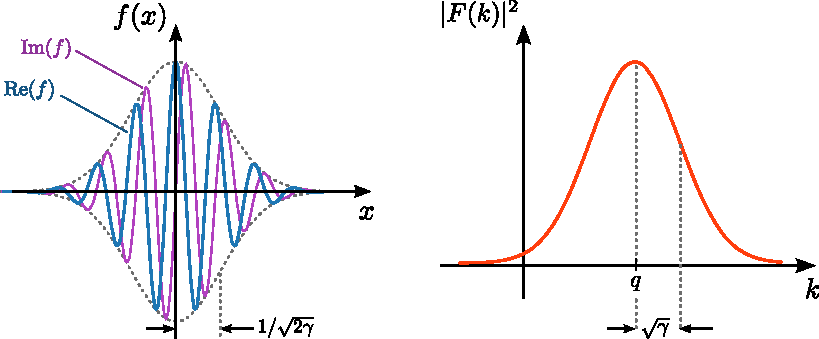
\includegraphics[width=0.75\textwidth]{fourier_example4}
\end{figure}

\subsection{The delta function}
\label{delta-function}

What happens when we feed the Fourier relations into one another?
Plugging the Fourier transform into the inverse Fourier transform,
\begin{align}
  f(x) &= \int_{-\infty}^\infty \frac{dk}{2\pi} \, e^{ikx} F(k) \\
  &= \int_{-\infty}^\infty \frac{dk}{2\pi} \, e^{ikx} \int_{-\infty}^\infty dx' e^{-ikx'} f(x')\\
  &= \int_{-\infty}^\infty dx' \left[ \int_{-\infty}^\infty \frac{dk}{2\pi} \, e^{ikx}  e^{-ikx'} \right] f(x').
\end{align}
Let us denote the term in brackets in the last line as
\begin{align}
  \delta(x-x') = \int_{-\infty}^\infty \frac{dk}{2\pi} \, e^{ik(x-x')}.
  \label{deltaxxp}
\end{align}
This is called the \textbf{delta function}. The delta function acts as
a kind of filter. When we multiply it by any function $f(x')$ and
integrate over $x'$, the result is the value of that function at a
particular point $x$:
\begin{align}
  \int_{-\infty}^\infty dx'\; \delta(x-x')\, f(x') = f(x).
\end{align}
But here's a problem: in Eq.~\eqref{deltaxxp}, the integrand does not
vanish at $\pm \infty$, so the integral is non-convergent!  We can get
around this by defining the delta function as a limiting case of a
convergent integral:
\begin{align}
  \delta(x-x') \equiv \lim_{\gamma \rightarrow 0} \, \int_{-\infty}^\infty \frac{dk}{2\pi} \, e^{ik(x-x')} \, e^{-\gamma k^2}.
\end{align}
The extra factor of $\exp(-\gamma k^2)$, which we have inserted into
the integrand, ensures that the integrand vanishes at $\pm \infty$,
making the integral convergent. As $\gamma \rightarrow 0$, this factor
goes to one, and the integrand approaches what we had before. But note
that the expression on the right is the Fourier transform for a
Gaussian wave-packet (see Section~\ref{gaussian-wave-packets}), so
\begin{align}
  \delta(x-x') \equiv \lim_{\gamma \rightarrow 0} \; \frac{1}{\sqrt{4\pi\gamma}} \, e^{-\frac{(x-x')^2}{4\gamma}}.
\end{align}
This is a Gaussian function of width $\sqrt{2\gamma}$ and area $1$.
Hence, the delta function can be regarded as the limit of a Gaussian
function as its width goes to zero while keeping the area under the
curve fixed at unity (which means the height of the peak goes to
infinity).

The ``filtering'' behavior of the delta function $\delta(x-x')$ can be
understood from its nature as an infinitesimal-width Gaussian. When we
multiply a function $f(x')$ by $\delta(x-x')$, the product is non-zero
only in the vicinity of $x' = x$. Since the area under the delta
function is unity, integrating that product over all $x'$ yields the
value of $f(x')$ at $x' = x$.

\begin{framed}\noindent
  \textit{Note}---In physics, the delta function is commonly used to
  represent the density distributions of point particles. For
  instance, the distribution of mass within an object can be
  represented by a mass density function.  Assuming one-dimensional
  space for simplicity, we define the mass density $\rho(x)$ as the
  mass per unit length at position $x$. By this definition,
  \begin{align}
    M = \int_{-\infty}^\infty \rho(x)\, dx
  \end{align}
  is the total mass of the object.  Now suppose the mass is distributed among $N$ point particles, which are located at distinct positions $x_1$, $x_2$, ..., $x_N$, and have masses $m_1$, $m_2$, ... $m_N$.  To describe this situation, we can write the mass density function as
  \begin{align}
    \rho(x) = \sum_{j=1}^N \, m_j\, \delta(x-x_j).
  \end{align}
  The reason for this is that if we integrate $\rho(x)$ around the
  vicinity of the $j$-th particle, the result is just the mass of that
  single particle, thanks to the features of the delta function:
  \begin{align}
    \lim_{\varepsilon\rightarrow 0^+}\, \int_{x_j - \varepsilon}^{x_j + \varepsilon} \rho(x) \, dx &= \sum_{i=1}^N m_i\; \Big[\lim_{\varepsilon\rightarrow 0^+}\, \int_{x_j - \varepsilon}^{x_j + \varepsilon} \delta(x-x_i) \,dx\Big]\\ &= \sum_{i=1}^N m_i\; \delta_{ij} \\ &= m_j.\end{align}
  Likewise, integrating $\rho(x)$ over all $x$ gives the total mass
  $m_1 + m_2 + \cdots + m_N$.
\end{framed}

\subsection{Multi-dimensional Fourier transforms (optional topic)}
\label{multi-dimensional-fourier-transforms}

When studying problems such as wave propagation, we often deal with
Fourier transforms of several variables.  This is conceptually
straightforward.  For a function $f(x_1, x_2, \dots, x_d)$ which
depends on $d$ independent spatial coordinates $x_1, x_2, \dots x_d$,
we can Fourier transform each coordinate individually:
\begin{align}
  F(k_1, k_2, \dots, k_d) = \int_{-\infty}^\infty dx_1\; e^{-ik_1x_1}\; \int_{-\infty}^\infty dx_2\; e^{-ik_2x_2}\,\cdots\, \int_{-\infty}^\infty dx_d\; e^{-ik_d x_d}\, f(x_1,x_2, \dots,x_N).
\end{align}
Each coordinate gets Fourier-transformed into its own independent $k$
variable, so the result is also a function of $d$ independent
variables.

We can express the multi-dimensional Fourier transform more compactly
using vector notation.  If $\vec{x}$ is a $d$-dimensional coordinate
vector, the Fourier-transformed coordinates can be written as
$\vec{k}$, and the Fourier transform is
\begin{align}
  F(\vec{k}) = \int d^d x \; \exp\left(-i\,\vec{k}\cdot\vec{x}\right) \, f\big(\vec{x}\big),
\end{align}
where $\int d^d x$ denotes an integral over the entire $d$-dimensional
space, and $\vec{k}\cdot\vec{x}$ is the usual dot product of two
vectors.  The inverse Fourier transform is
\begin{align}
  f(\vec{x}) = \int \frac{d^dk}{(2\pi)^d}\; \exp\left(i\,\vec{k}\cdot\vec{x}\right)\, F\big(\vec{k}\big).
\end{align}
The delta function can also be defined in $d$-dimensional space, as
the Fourier transform of a plane wave:
\begin{align}
  \delta^d(\vec{x}-\vec{x}') = \int \frac{d^dk}{(2\pi)^d} \, \exp\left[i\vec{k} \cdot \left(\vec{x}-\vec{x}'\right)\right].
\end{align}
Note that $\delta^d$ has the dimensions of $[x]^{-d}$.  The
multi-dimensional delta function has a filtering property similar to
the one-dimensional delta function. For any $f(x_1,\dots,x_d)$,
\begin{align}
  \int d^dx \; \delta^d(\vec{x}-\vec{x}') \, f(\vec{x}) = f(\vec{x}').
\end{align}

\subsection{Exercises}\label{exercises}

\begin{enumerate}
\item
  Find the relationship between the coefficients
  $\{\alpha_n, \beta_m\}$ in the sine/cosine Fourier series and the
  coefficients $f_n$ in the complex exponential Fourier
  series:
  \begin{align}
    f(x) &= \sum_{n=1}^\infty \alpha_n \sin\left(\frac{2\pi n x}{a}\right) + \sum_{m=0}^\infty \beta_m \cos\left(\frac{2 \pi m x}{a}\right) \\
    &= \sum_{n=-\infty}^\infty f_n \exp\left(\frac{2\pi i n x}{a}\right).
  \end{align}

\item
  Consider the triangular wave
  \begin{equation}
    f(x) = \left\{\begin{array}{rr}- x, &-a/2 \le x < 0, \\
    x, & 0 \le x < a/2\end{array}\right.
  \end{equation}

  \begin{enumerate}[(a)]
  \item
    Derive the Fourier series expansion.

  \item
    Plot the Fourier series numerically, and show that it converges to
    the triangular wave as the number of terms increases.
  \end{enumerate}

\item
  A periodic function $f(x)$ (with period $a$) is written as a complex
  Fourier series with coefficients $\{f_0, f_{\pm1}, f_{\pm2},
  \dots\}$. Determine the relationship(s) between the Fourier
  coefficients under each of the following scenarios:
  \begin{enumerate}[(a)]
  \item $f(x)$ is real for all $x$.
  \item $f(x) = f(-x)$ for all $x$
  \item $f(x) = f(-x)^*$ for all $x$.
  \hfill{\scriptsize [solution~available]}
  \end{enumerate}

\item
  Prove the properties of the Fourier transform listed in
  Section~\ref{fourier-basic-properties}.

\item
  Find the Fourier transform of $f(x) = \sin(\kappa x)/x.$

\item
  Prove that if $f(x)$ is a real function, then its Fourier transform
  satisfies $F(k) = F(-k)^*$.

\item
  Prove that
  \begin{equation}
    \delta(ax) = \frac{1}{a}\,\delta(x),
  \end{equation}
  where $a$ is any nonzero real number.
  \hfill{\scriptsize [solution~available]}

\item Calculate
  \begin{equation}
    \int_{-\infty}^\infty dx \int_{-\infty}^\infty dy \;
    x^2\, \delta\left(\sqrt{x^2+y^2}-a\right),
  \end{equation}
  where $a$ is a real number.
  \hfill{\scriptsize [solution~available]}
  
\item
  Consider the integral $$I = \int_{-\infty}^\infty e^{-\gamma\left(x
    + i\lambda\right)^2} \; dx,$$ where $\gamma \in \mathbb{R}^+$ and
  $\lambda \in \mathbb{R}.$ (This is the Gaussian integral with an
  imaginary displacement in the integration variable, which we
  encountered while discussing Gaussian wave-packets
  (Section~\ref{gaussian-wave-packets}).  To solve this integral,
  consult the contour shown in the figure below (for the case $\lambda
  > 0$):

  \begin{figure}[ht]
    \centering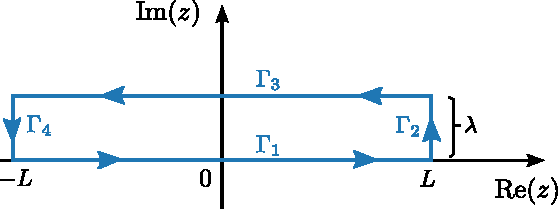
\includegraphics[width=0.6\textwidth]{rectangular_contour}
  \end{figure}

  Show, by parameterization, that
  \begin{enumerate}[(i)]
  \item $\displaystyle I = - \lim_{L\rightarrow \infty} \int_{\Gamma_3} e^{-\gamma
    z^2} dz$, and
  \item $\displaystyle \lim_{L\rightarrow \infty} \int_{\Gamma_2~\text{or}~\Gamma_4}
  e^{-\gamma z^2}\, dz = 0.$
  \end{enumerate}
  Hence, explain why $I = \sqrt{\pi/\gamma}.$

\item A \textbf{dispersive wave medium} is one in which the frequency
  of a plane wave is not proportional to its wave-vector.  For 1D
  space, consider a wavefunction $f(x,t)$, which at time $t = 0$ has
  the form
  \begin{equation}
    f(x, 0) = \int_{-\infty}^\infty dk \; e^{-\alpha(k-k_0)^2} \, e^{ikx},
    \label{fx0}
  \end{equation}
  for some $\alpha \in \mathbb{R}^+$ and $k_0 \in \mathbb{R}$.  Based
  on the discussion in Section~\ref{gaussian-wave-packets}, $f(x,0)$
  can be shown to be a Gaussian wave-packet.  But we can also intepret
  the integral in Eq.~\eqref{fx0} as a superposition of plane waves
  $\exp(ikx)$, for various $k$.  Away from $t = 0$, each plane wave
  naturally generalizes to $\exp[i(kx - \omega t)]$, so
  \begin{equation}
    f(x, t) = \int_{-\infty}^\infty dk \; e^{-\alpha(k-k_0)^2} \, e^{i[kx-\omega t]}. \label{fxt_wavepacket}
  \end{equation}
  Now suppose $\omega$ is some arbitrarily complicated function of
  $k$.  For $k \approx k_0$, take the Taylor expansion
  \begin{equation}
    \omega \approx \omega_0 + v_g (k-k_0) + \cdots,
    \;\;\; \mathrm{where}\;\;
    v_g \equiv \left[\frac{d\omega}{dk}\right]_{k=k_0}.
    \label{dispersion}
  \end{equation}
  By solving the integral \eqref{fxt_wavepacket}, prove that $f(x, t)$
  has the form of a Gaussian wave-packet whose center moves with
  velocity $v_g$ (called the \textbf{group velocity}).

  Next, show that if the Taylor expansion in Eq.~\eqref{dispersion}
  has a non-vanishing second-order term, then the wave-packet spreads
  (or ``disperses'') with increasing $t$.
  
\end{enumerate}
    


\end{document}
